%% LICENCE: CC-BY-NC-SA
%% Copyright: Jesús Espino
%% Based on Git Internals chapter of ProGit book (http://git-scm.com/book)
\documentclass[10pt]{beamer}

\usepackage[utf8]{inputenc}
\usepackage[spanish]{babel}
\usepackage{graphicx}

\mode<presentation>
\usetheme{Madrid}
%\usecolortheme[RGB={111,73,135}]{structure}
\usecolortheme[RGB={128,0,0}]{structure}
%\usecolortheme[RGB={0,96,0}]{structure}
%\usecolortheme[RGB={200,0,200}]{structure}
%\usecolortheme[RGB={0,128,0}]{structure}
%\usecolortheme[RGB={0,0,128}]{structure}
\usefonttheme{serif}
\useinnertheme{rectangles}
\useoutertheme{split}

\setbeamercovered{transparent}

\title{Git Internals}
\author{Jesús Espino García}
\date{19 de Abril de 2013}
\subject{Git Internals}

\institute[Kaleidos]{jesus.espino@kaleidos.net\\@jespinog\\
\includegraphics[height=1.5cm]{kaleidos.png}}

\setcounter{tocdepth}{2}

\AtBeginSubsection[]
{
  \begin{frame}[containsverbatim]<beamer>{Indice}
    \tableofcontents[sectionstyle=show/shaded,subsectionstyle=show/shaded/hide]
  \end{frame}
}

\begin{document}

  \frame{\maketitle}

  \section*{Introducción}

  \begin{frame}[containsverbatim]
    \frametitle{Introducción}
    \begin{itemize}
      \item Python 3.3
      \item Usaré ctypes para los ejemplos.
      \item La estructura de un objeto en cpython.
      \item Los objetos escritos en c de python.
      \item El proceso de creación de un nuevo objeto.
    \end{itemize}
  \end{frame}

  \section*{Definiciones}

  \begin{frame}[containsverbatim]
    \frametitle{¿Qué es un tipo en python?}
    \begin{itemize}
      \item Un tipo es una clase
      \item Es una estructura compuesta de datos y slots
      \item Los slots son punteros a funciones que definen comportamientos
      \item Los tipos son objetos de python
      \item Los tipos son de objetos de tipo tipo
    \end{itemize}
  \end{frame}

  \begin{frame}[containsverbatim]
    \frametitle{¿Qué es un tipo en python?}
    \begin{verbatim}
>>> class Prueba:
...   pass
...
>>> type(Prueba)
<class 'type'>
>>> isinstance(Prueba, object)
True
>>> isinstance(type, object)
True
>>> type(type)
<class 'type'>
    \end{verbatim}
  \end{frame}

  \begin{frame}[containsverbatim]
    \frametitle{¿Qué es una instancia?}
    \begin{itemize}
      \item Es exactamente lo mismo que un objeto.
      \item Es una zona reservada de la memoria con datos.
      \item Tiene un tipo (y solo 1) que determina qué puede hacer el objeto.
      \item El tipo de un objeto no cambia a lo largo de su vida (existen excepciones).
    \end{itemize}
  \end{frame}

  \begin{frame}[containsverbatim]
    \frametitle{¿Qué es una instancia?}
    \begin{verbatim}
>>> prueba = Prueba()
>>> type(prueba)
<class '__main__.Prueba'>
>>> prueba
<__main__.Prueba object at 0x7f3555af9bd0>
>>> Prueba
<class '__main__.Prueba'>
>>> id(prueba)
139867047566288
>>> hex(id(prueba))
'0x7f3555af9bd0'
    \end{verbatim}
  \end{frame}

  \begin{frame}[containsverbatim]
    \frametitle{Diagrama de herencia}
    \begin{center}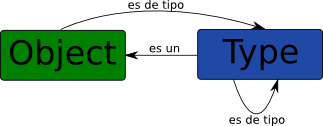
\includegraphics{img/Object-Type-Relation.png}\end{center}
  \end{frame}

  \begin{frame}[containsverbatim]
    \frametitle{Diagrama de herencia}
    \begin{center}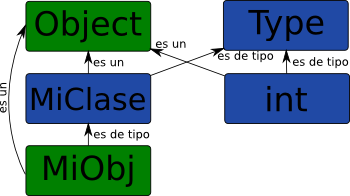
\includegraphics{img/MyClass-BuiltinClass-Relation.png}\end{center}
  \end{frame}

  \begin{frame}[containsverbatim]
    \frametitle{Diagrama de herencia}
    \begin{center}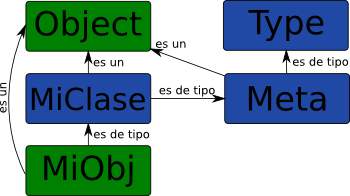
\includegraphics{img/Metaclass-Relation.png}\end{center}
  \end{frame}

  \section*{Estructura de objetos}

  \begin{frame}[containsverbatim]
    \frametitle{Estructura básica de un objetos}
    \begin{center}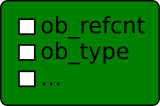
\includegraphics{img/PyObject.png}\end{center}
    \begin{itemize}
      \item \verb+ob_refcnt+: contador de referencias
      \item \verb+ob_type+: puntero al tipo de datos
      \item Otros datos específicos para este tipo
    \end{itemize}
  \end{frame}

  \begin{frame}[containsverbatim]
    \frametitle{Estructura variable básica de un objetos}
    \begin{center}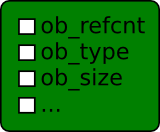
\includegraphics{img/PyVarObject.png}\end{center}
    \begin{itemize}
      \item \verb+ob_refcnt+: contador de referencias
      \item \verb+ob_type+: puntero al tipo de datos
      \item \verb+ob_size+: tamaño del objeto
      \item Otros datos específicos para este tipo
    \end{itemize}
  \end{frame}

  \section*{Tipos en CPython}

  \begin{frame}[containsverbatim]
    \frametitle{El objeto None}
    \begin{center}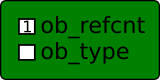
\includegraphics{img/None.png}\end{center}
    \begin{itemize}
      \item Es el tipo más simple
      \item Su instancia es singleton
      \item No añade ningún dato extra a la estructura básica de objeto
    \end{itemize}
  \end{frame}

  \begin{frame}[containsverbatim]
    \frametitle{Very bad things}
    \begin{verbatim}
>>> ref_cnt = ctypes.c_long.from_address(id(None))
>>> ref_cnt.value = 0
Fatal Python error: deallocating None

Current thread 0x00007f2fb8d2a700:
  File "<stdin>", line 1 in <module>
[2]    10960 abort (core dumped)  python3
    \end{verbatim}
  \end{frame}

  \begin{frame}[containsverbatim]
    \frametitle{El objeto int}
    \begin{center}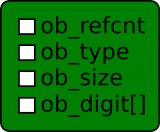
\includegraphics{img/Int.png}\end{center}
    \begin{itemize}
      \item \verb+ob_digit+: array de enteros
      \item El valor del entero es \verb+sum(map(lambda x: 1024*1024*1024, ob_size))+
    \end{itemize}
  \end{frame}

  \begin{frame}[containsverbatim]
    \frametitle{El objeto int}
    \begin{center}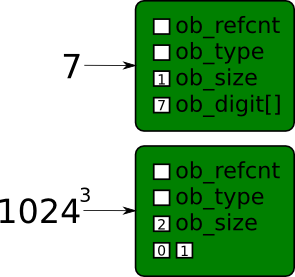
\includegraphics{img/Int-Usage.png}\end{center}
  \end{frame}

  \begin{frame}[containsverbatim]
    \frametitle{El objeto int}
    \begin{verbatim}
>>> longsize = ctypes.sizeof(ctypes.c_long)
>>> intsize = ctypes.sizeof(ctypes.c_int)
>>> x = 100
>>> ctypes.c_long.from_address(id(x) + longsize * 2)
c_long(1)
>>> ctypes.c_uint.from_address(id(x) + longsize * 3)
c_uint(100)
>>> x = 1024 * 1024 * 1024
>>> ctypes.c_long.from_address(id(x) + longsize * 2)
c_long(2)
>>> ctypes.c_uint.from_address(id(x) + longsize * 3)
c_uint(0)
>>> ctypes.c_uint.from_address(id(x) + longsize * 3 + intsize)
c_uint(1)
    \end{verbatim}
  \end{frame}

  \begin{frame}[containsverbatim]
    \frametitle{Very bad things}
    \begin{verbatim}
>>> longsize = ctypes.sizeof(ctypes.c_long)
>>> x = 1000
>>> int_value = ctypes.c_uint.from_address(id(x) + longsize * 3)
>>> int_value.value = 1001
>>> x
1001
>>> 1000
1000
    \end{verbatim}
  \end{frame}

  \begin{frame}[containsverbatim]
    \frametitle{Very bad things}
    \begin{verbatim}
>>> longsize = ctypes.sizeof(ctypes.c_long)
>>> x = 100
>>> int_value = ctypes.c_uint.from_address(id(x) + longsize * 3)
>>> int_value.value = 101
>>> x
101
>>> 100
101
>>> 100 + 2
103
    \end{verbatim}
  \end{frame}

  \begin{frame}[containsverbatim]
    \frametitle{El objeto bool}
    \begin{center}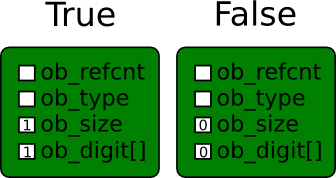
\includegraphics{img/True-False.png}\end{center}
    \begin{itemize}
      \item Realmente son 2 instancias int con un tipo específico y valores 0 y 1
    \end{itemize}
  \end{frame}

  \begin{frame}[containsverbatim]
    \frametitle{El objeto bool}
    \begin{verbatim}
>>> longsize = ctypes.sizeof(ctypes.c_long)
>>> ctypes.c_long.from_address(id(True) + longsize * 2)
c_long(1)
>>> ctypes.c_uint.from_address(id(True) + longsize * 3)
c_uint(1)
>>> ctypes.c_long.from_address(id(False) + longsize * 2)
c_long(0)
>>> ctypes.c_uint.from_address(id(False) + longsize * 3)
c_uint(0)
    \end{verbatim}
  \end{frame}

  \begin{frame}[containsverbatim]
    \frametitle{Very bad things}
    \begin{verbatim}
>>> val = ctypes.c_int.from_address(id(True) + longsize * 2)
>>> val.value = 0
>>> val = ctypes.c_int.from_address(id(True) + longsize * 3)
>>> val.value = 0
>>> True == False
True
    \end{verbatim}
  \end{frame}

  \begin{frame}[containsverbatim]
    \frametitle{El objeto float}
    \begin{center}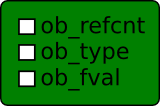
\includegraphics{img/Float.png}\end{center}
    \begin{itemize}
      \item \verb+ob_fval+: es un double
    \end{itemize}
  \end{frame}

  \begin{frame}[containsverbatim]
    \frametitle{El objeto float}
    \begin{verbatim}
>>> longsize = ctypes.sizeof(ctypes.c_long)
>>> x = 1.5
>>> ctypes.c_double.from_address(id(x) + longsize * 2)
c_double(1.5)
    \end{verbatim}
  \end{frame}

  \begin{frame}[containsverbatim]
    \frametitle{El objeto complex}
    \begin{center}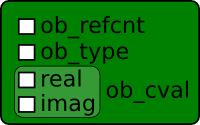
\includegraphics{img/Complex.png}\end{center}
    \begin{itemize}
      \item \verb+cval+: dos valores double \verb+real+ e \verb+imag+
    \end{itemize}
  \end{frame}

  \begin{frame}[containsverbatim]
    \frametitle{El objeto complex}
    \begin{verbatim}
>>> longsize = ctypes.sizeof(ctypes.c_long)
>>> doublesize = ctypes.sizeof(ctypes.c_double)
>>> x = 1 + 3j
>>> ctypes.c_double.from_address(id(x) + longsize * 2)
c_double(1.0)
>>> ctypes.c_double.from_address(id(x) + longsize * 2 + doublesize)
c_double(3.0)
    \end{verbatim}
  \end{frame}

  \begin{frame}[containsverbatim]
    \frametitle{Referencias}
    \begin{itemize}
      \item \small{http://git-scm.com/ - Web oficial de git.}
      \item \small{http://git-scm.com/book - ProGit (El libro de Git).}
      \item \small{Documentation/technical - Technical doc in the git respoitory. }
      \item \small{http://gitguys.com/ - Página sobre git.}
      \item \small{http://github.com/ - Servicio de git por excelencia.}
      \item \small{http://bitbucket.org/ - Servicio de git de repositorios privados gratis.}
    \end{itemize}
  \end{frame}

  \begin{frame}[containsverbatim]
    \frametitle{Dudas}
    \dots
  \end{frame}

\end{document}
